\chapter{Introduction}

LEXenstein is a framework for Lexical Simplification. It contains several methods, tools and resources for one to easily create Lexical Simplification systems and test them in various distinct ways. It takes Lexical Simplification as a process that can be modeled as a pipeline of sub-processes, as illustrated in Figure~\ref{fig:exlepipe}.

\begin{figure}[htbp!] 
\centering    
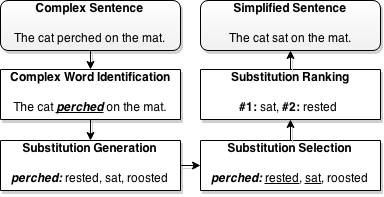
\includegraphics[scale=0.8]{Figs/diagramshadow.png}
\caption{Lexical Simplification pipeline}
\label{fig:exlepipe}
\end{figure}

Each task in Figure~\ref{fig:exlepipe} can be described as:

\begin{enumerate}
\item \textbf{Complex Word Identification}: Task of deciding which words of a given sentence may not be understood by a given target audience and hence must be simplified.

\item \textbf{Substitution Generation}: Task of finding pairs of words or expressions that share the same meaning and are interchangeable in some context.

\item \textbf{Substitution Selection}: Task of deciding which is the meaning of a given complex ambiguous word in a sentence to be simplified, and then selecting which substitutions available also represent that meaning.

\item \textbf{Substitution Ranking}: Task of ranking the remaining substitutions of a given complex word by their simplicity.
\end{enumerate}

Its name is a reference to the \textit{Frankenstein} novel, published by \cite{frankenstein}. It refers to the fact that one can, as Victor Frankenstein did, create an entire Lexical Simplification ``creature'' by combining multiple ``pieces'' of the Lexical Simplification pipeline together.

LEXenstein is divided in several modules: Complex Word Identification, Substitution Generation, Substitution Selection, Substitution Ranking, Feature Estimation, Evaluation, Text Adorning, Spelling Correction and Utilities. In the next Sections, we describe the VICTOR and CWICTOR file formats, explain how to properly setup LEXenstein, and discuss in detail the components included in each module of the framework.